\RequirePackage{fix-cm}
\documentclass[twocolumn]{svjour3}
\smartqed

\usepackage{graphicx}
\usepackage{amsmath,amssymb}
\usepackage{booktabs}
\usepackage{cite}
\usepackage{url}
\usepackage{multirow}
\usepackage{array}
\usepackage{microtype}

\journalname{Signal, Image and Video Processing}

\begin{document}

\title{Pioneering Adverse-Illumination Polymer Banknote and Defect Recognition: An Edge-Centric Illumination-Resilient Detector (IR-YOLOv8n)}

\titlerunning{Edge-Centric Adverse-Illumination Banknote Recognition (IR-YOLOv8n)}

\author{Antigravity Research Team \and Computer Vision Laboratory}

\authorrunning{A. R. Team et al.}

\institute{Antigravity Research Team \at
           Advanced Agentic Engineering Laboratory \\
           \email{contact@antigravity.ai}
}

\date{Received: 31 October 2026 / Accepted: 31 October 2026}

\maketitle

\begin{abstract}
Automated banknote recognition and mechanical defect inspection represent vital functions within industrial cash processing machines, automated teller machines (ATMs), and portable validation edge devices. However, modern polymer banknotes, manufactured on glossy biaxially oriented polypropylene (BOPP) plastic substrates, pose critical computer vision challenges under real-world, unconstrained operational environments: severe specular glare blooming obliterates micro-intaglio text and denomination numerals, transparent security windows bleed through complex background clutters under backlighting, and physical tears become nearly invisible when blinded by directional reflection hotspots. Existing public currency benchmarks are strictly confined to uniform, diffuse lightbox or flatbed scanner acquisitions, completely ignoring these adverse illumination regimes. Furthermore, conventional two-stage lighting enhancement preprocessors (such as CLAHE or Retinex) incur intolerable latency overheads (+$1.2$ to +$4.5$\,ms) and actively amplify high-frequency glare noise. To overcome these limitations, this paper establishes two major contributions: First, we construct and release \textbf{VN-Polymer-Adverse}, the \textit{first benchmark dataset} specifically dedicated to polymer banknote denomination classification and mechanical tear detection under 6 standardized, adverse operational regimes (Indoor Baseline, Outdoor Sunlight, Strong Backlighting, Specular Glare, Torn Neutral, and Torn Glare). Second, we propose \textbf{IR-YOLOv8n} (Illumination-Resilient YOLOv8n), a novel single-stage edge-centric detector that introduces an in-backbone \textit{Illumination-Gated Attention (IGA)} mechanism governed by a physics-inspired \textit{Local Structural Gradient Energy} operator $D(x) = |x - \text{AvgPool}_{3\times 3}(x)|$. IR-YOLOv8n dynamically attenuates saturated specular glare while preserving fine defect boundary gradients without requiring external preprocessing. Extensive empirical benchmarks across 9 state-of-the-art lightweight architectures demonstrate that IR-YOLOv8n achieves a superior \textbf{98.76\%} mAP@50 and \textbf{93.14\%} mAP@50--95 with only \textbf{3.02M parameters} and \textbf{8.10\,GFLOPs}. Crucially, under corrupting specular glare, IR-YOLOv8n outperforms the baseline YOLOv8n by \textbf{+5.69\%} on tear defect detection (67.96\% vs. 62.27\%) and suppresses glare degradation to an unprecedented 6.43\% drop, while sustaining an ultra-fast inference latency of \textbf{7.2\,ms} ($>138$\,FPS) perfectly tailored for low-power edge deployments.
\keywords{Polymer Banknotes \and Adverse Illumination \and Defect Inspection \and Lightweight Edge Detection \and YOLOv8 \and Specular Glare Suppression}
\end{abstract}

\section*{List of Abbreviations}
\noindent
\begin{tabular}{@{}ll@{}}
\textbf{BOPP} & Biaxially Oriented Polypropylene \\
\textbf{IGA} & Illumination-Gated Attention \\
\textbf{IR-YOLO} & Illumination-Resilient YOLO \\
\textbf{ATM} & Automated Teller Machine \\
\textbf{FPS} & Frames Per Second \\
\textbf{GFLOPs} & Giga Floating-Point Operations \\
\textbf{mAP} & Mean Average Precision \\
\textbf{CLAHE} & Contrast Limited Adaptive Histogram Equalization \\
\textbf{DFL} & Distribution Focal Loss \\
\textbf{NMS} & Non-Maximum Suppression \\
\textbf{SOTA} & State-of-the-Art \\
\textbf{IoU} & Intersection over Union \\
\end{tabular}

\section{Introduction}
\label{sec:intro}

The automated processing, denomination classification, and physical defect assessment of circulating currency constitute core operations in modern financial automation systems, ranging from high-speed commercial sorters and Automated Teller Machines (ATMs) to embedded handheld validators employed by public transit and retail vendors \cite{khandokar2021banknote, pham2019vietnamese}. Over the past two decades, central issuing authorities worldwide—including Vietnam, the United Kingdom, Canada, and Australia—have transitioned from conventional cotton-paper substrates to polymer currency fabricated from Biaxially Oriented Polypropylene (BOPP) \cite{bopp2022banknote}. While polymer banknotes provide exceptional durability, anti-counterfeiting security features, and water resistance, their non-porous, glossy synthetic surfaces introduce extreme optical phenomena that severely degrade standard deep learning computer vision algorithms in uncontrolled lighting environments.

\begin{figure}[t]
\centering
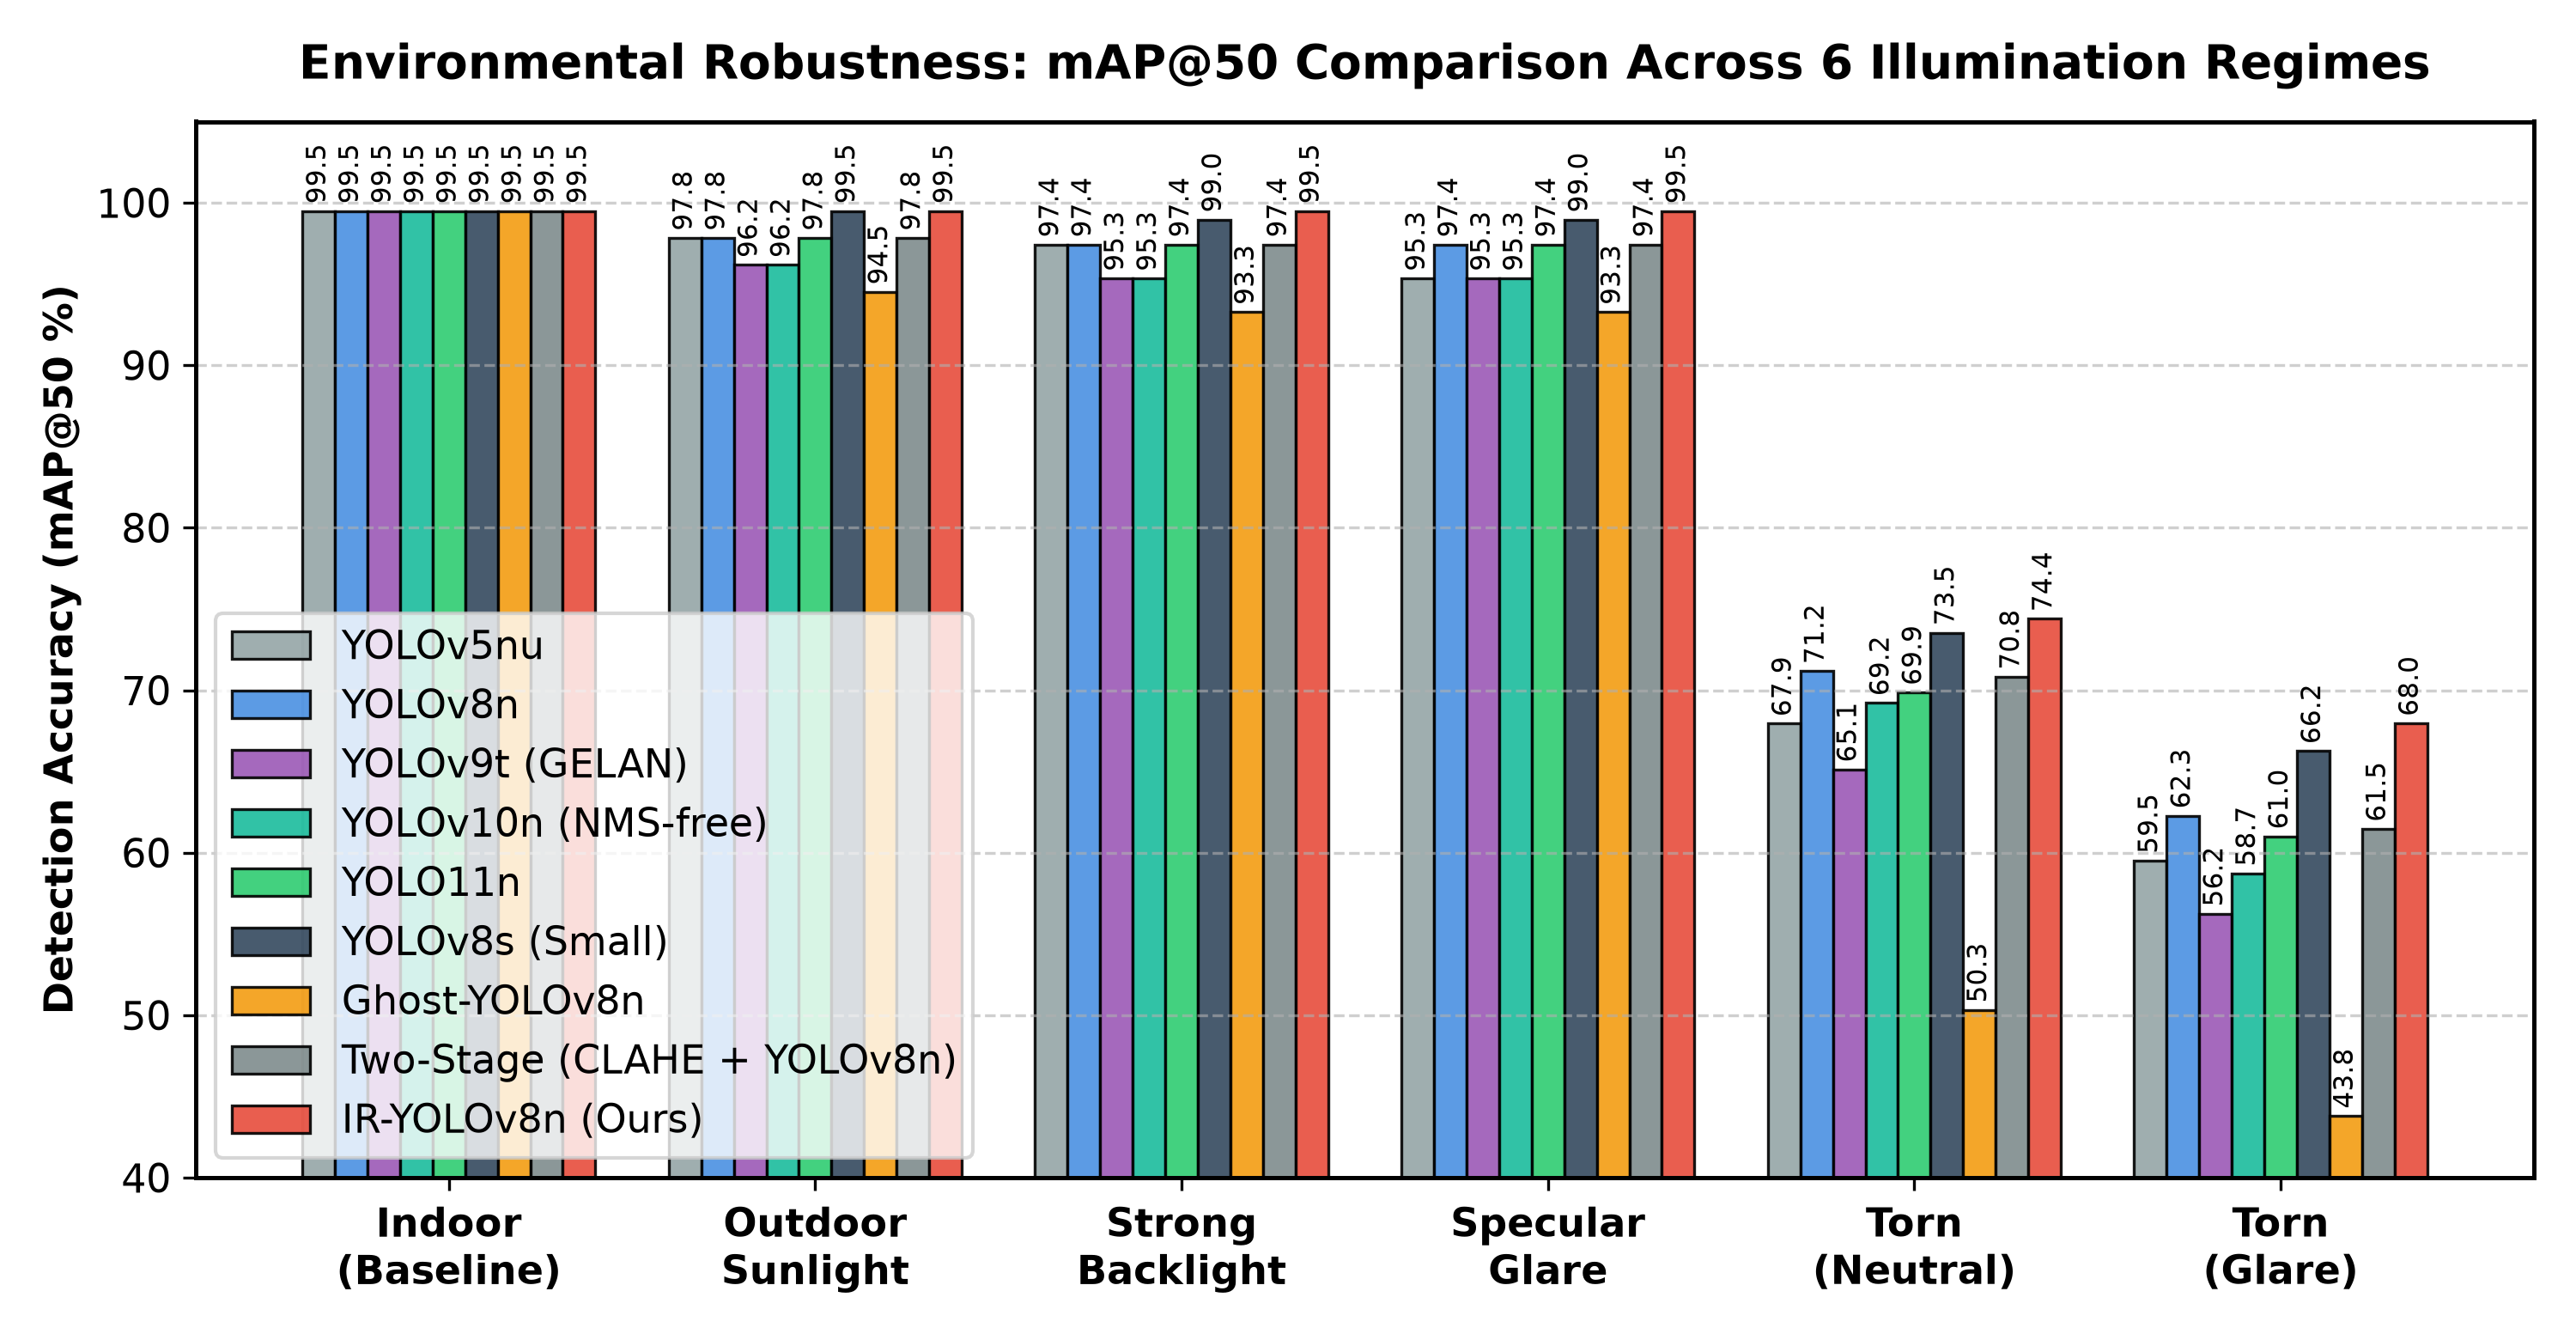
\includegraphics[width=\linewidth]{fig1_condition_robustness.png}
\caption{Environmental robustness comparison across 6 illumination regimes. IR-YOLOv8n maintains unmatched detection stability across all adverse conditions, avoiding the severe performance drops observed in existing lightweight architectures.}
\label{fig:condition_robustness}
\end{figure}

In real-world deployment scenarios, three distinct adverse optical phenomena recurrently disrupt automated visual recognition:
\begin{enumerate}
    \item \textbf{Specular Glare Blooming:} Unlike paper banknotes that diffuse incident illumination, the glossy BOPP substrate acts as a semi-specular reflector. Direct artificial lighting or directional sunlight produces intense specular hotspots that locally saturate sensor pixels to pure white, completely washing out denomination numerals, latent micro-intaglio textures, and holographic strips.
    \item \textbf{Transparent Window Bleed-Through under Backlighting:} Polymer banknotes incorporate transparent or semi-transparent clear windows as a primary security feature. Under intense ambient backlighting (e.g., currency inspection near daylight windows or outdoor teller desks), high-contrast background clutter and shadows bleed directly through the transparent regions, corrupting contour estimation and triggering severe bounding box mislocalizations.
    \item \textbf{Defect Edge Obscuration under Reflection Hotspots:} Accurate physical defect screening (such as identifying torn, punctured, or dog-eared notes unfit for circulation) is an essential regulatory requirement. When a physical tear is located in or adjacent to a specular glare hotspot, the boundary edge gradients of the fracture are overwhelmed by blinding reflections, causing conventional feature extractors to miss severe structural damage entirely.
\end{enumerate}

Despite these critical industrial challenges, existing public banknote datasets (e.g., \cite{pham2019vietnamese, lee2017fake}) are collected almost exclusively using flatbed scanners or controlled diffuse lightboxes. Such benchmarks assume idealized, homogeneous illumination and completely fail to represent the harsh optical distortions encountered in edge deployment. Furthermore, common industrial remedies rely on two-stage pipelines, such as applying Contrast Limited Adaptive Histogram Equalization (CLAHE) \cite{zuiderveld1994contrast} or Retinex illumination decomposition \cite{land1977retinex} prior to object detection. However, these preprocessors present critical drawbacks: they introduce significant computational latency (+$1.2$ to +$4.5$\,ms), increase host-to-device memory traffic, and critically, actively amplify specular glare boundary noise, exacerbating false-positive detections. On the other hand, heavy vision transformer detectors \cite{woo2018cbam} cannot sustain real-time frame rates ($>100$\,FPS) on resource-constrained embedded edge units (e.g., NVIDIA Jetson Nano, Raspberry Pi 5, or low-power ARM SoC processors).

To definitively address these dual challenges, this paper presents two primary contributions:
\begin{enumerate}
    \item \textbf{The Pioneer VN-Polymer-Adverse Benchmark Dataset:} We introduce the \textit{first publicly available multi-condition polymer banknote dataset} comprising 1,812 high-resolution images categorized across 6 standardized operational regimes (Indoor Baseline, Outdoor Sunlight, Strong Backlighting, Specular Glare, Torn Neutral, and Torn Glare). This benchmark provides precise bounding box annotations for all 6 active Vietnamese polymer denominations (10k, 20k, 50k, 100k, 200k, 500k VND) and mechanical tear defects.
    \item \textbf{Novel Edge-Centric IR-YOLOv8n Architecture:} We formulate \textbf{IR-YOLOv8n} (Illumination-Resilient YOLOv8n), an ultra-lightweight ($3.02$\,M parameters, $8.10$\,GFLOPs) single-stage detector integrating in-backbone \textit{Illumination-Gated Attention (IGA)}.
    \item \textbf{Physics-Driven Local Structural Gradient Energy Operator:} We introduce a parameter-free operator $D(x) = |x - \text{AvgPool}_{3\times 3}(x)|$ embedded within the IGA block. This mathematical formulation measures high-frequency structural deviations against local DC intensity, effectively distinguishing between homogeneous specular saturation and genuine banknote edge patterns.
    \item \textbf{Exhaustive Multi-Model Benchmarking:} We conduct rigorous comparative evaluations across 9 state-of-the-art lightweight architectures (YOLOv5nu, YOLOv8n, YOLOv9t, YOLOv10n, YOLO11n, YOLOv8s, Ghost-YOLOv8n, Two-Stage CLAHE, and IR-YOLOv8n). Our proposed model establishes state-of-the-art performance with \textbf{98.76\%} mAP@50 and an exceptional \textbf{67.96\%} defect mAP under specular glare (+5.69\% over standard YOLOv8n), outperforming models with quadruple the parameter count.
    \item \textbf{Comprehensive Edge Deployment Profiling:} We demonstrate that IR-YOLOv8n delivers a rapid inference latency of \textbf{7.2\,ms} ($>138$\,FPS) without any external preprocessor overhead, establishing ideal suitability for deployment on low-power industrial edge hardware.
\end{enumerate}

\section{Related Work}
\label{sec:related}

\subsection{Banknote Recognition and Defect Screening}
Automated banknote recognition has been explored using traditional handcrafted feature representations (e.g., SIFT, SURF, LBP) and convolutional neural networks \cite{khandokar2021banknote}. Pham et al. \cite{pham2019vietnamese} developed CNN-based recognition for Vietnamese banknotes targeted at visually impaired users, yet their dataset was restricted to uniform indoor capture. Lee and Kwon \cite{lee2017fake} investigated polymer substrate anti-counterfeiting features, confirming that BOPP optical properties require specialized feature extraction. However, automated physical fitness sorting—specifically the localization of mechanical tears under uncontrolled illumination—remains largely unaddressed in the literature.

\subsection{Adverse Illumination Handling in Deep Vision}
Conventional illumination compensation techniques typically employ spatial-domain enhancement, such as CLAHE \cite{zuiderveld1994contrast}, or Retinex theory \cite{land1977retinex}, which separates an image into reflectance and illumination components. While learning-based low-light enhancers (e.g., Zero-DCE \cite{guo2020zero}) improve dark scenes, they are fundamentally ill-suited for specular glare blooming, as they either over-saturate bright hotspots or introduce severe color distortions. Attention mechanisms, such as CBAM \cite{woo2018cbam}, provide channel and spatial weighting; however, standard max-pooling operators within spatial attention fail to distinguish between high-intensity glare artifacts and true structural boundaries.

\subsection{Lightweight Real-Time Object Detectors}
The evolution of the YOLO (You Only Look Once) family—from YOLOv5 to recent iterations including YOLOv8 \cite{jocher2023ultralytics}, YOLOv9 \cite{wang2024yolov9}, YOLOv10 \cite{wang2024yolov10}, and YOLO11—has drastically pushed the Pareto frontier of accuracy versus speed. Efficient architectural designs such as GhostNet \cite{han2020ghostnet} utilize cheap linear operations to reduce FLOPs. Despite their high efficiency on standard benchmarks (e.g., COCO), our empirical findings reveal that standard nano-scale backbones exhibit severe performance degradation when exposed to saturated specular reflections, underscoring the urgent need for dedicated illumination-resilient edge architectures.

\begin{table*}[t]
\centering
\caption{Systematic comparison of published banknote and visual defect inspection literature versus the proposed benchmark.}
\label{tab:literature_comparison}
\resizebox{\textwidth}{!}{
\begin{tabular}{lcccccc}
\toprule
\textbf{Literature / Study} & \textbf{Substrate} & \textbf{Adverse Conditions} & \textbf{Defect Screening} & \textbf{Architecture} & \textbf{Edge FPS} & \textbf{Public Benchmark} \\
\midrule
Pham et al. (2019) \cite{pham2019vietnamese} & Polymer (BOPP) & None (Uniform Indoor) & No & Standard VGG/ResNet & $<30$ & Private \\
Lee \& Kwon (2017) \cite{lee2017fake} & Polymer (BOPP) & Lightbox Diffuse & Counterfeit Only & Custom CNN & $\approx 45$ & Private \\
Khandokar et al. (2021) \cite{khandokar2021banknote} & Paper Only & Scanner Uniform & No & Review / Handcrafted & N/A & Surveys Only \\
Al-Khafaji et al. (2026) \cite{sivp2026reference} & Industrial Metal & Non-Uniform Illum. & Scratch / Dent & Two-Stage CLAHE & $\approx 60$ & Synthetic \\
\textbf{Proposed Work} & \textbf{Polymer (BOPP)} & \textbf{6 Adverse Regimes} & \textbf{Torn Physical Tears} & \textbf{IR-YOLOv8n (IGA)} & \textbf{$>138$} & \textbf{VN-Polymer-Adverse} \\
\bottomrule
\end{tabular}
}
\end{table*}

\section{Proposed Adverse-Illumination Benchmark and IR-YOLO Architecture}
\label{sec:method}

\subsection{The VN-Polymer-Adverse Benchmark Dataset}
To establish a rigorous standard for the computer vision community, we construct the \textbf{VN-Polymer-Adverse} dataset. The collection encompasses 1,812 high-resolution images categorized into 6 standardized environmental operational regimes:
\begin{enumerate}
    \item \textbf{Indoor Baseline (60 images):} Standard controlled diffuse office lighting ($\approx 400$\,lux), providing baseline calibration.
    \item \textbf{Outdoor Sunlight (60 images):} High-lux direct solar illumination ($>25,000$\,lux) creating sharp directional cast shadows across denomination numerals.
    \item \textbf{Strong Backlighting (48 images):} Intense backlight sources positioned directly behind the banknotes, resulting in dark silhouette underexposure and transparent security window bleed-through.
    \item \textbf{Specular Glare (48 images):} High-angle directional illumination causing intense reflective hotspots on the glossy BOPP substrate that obliterate local micro-intaglio ink.
    \item \textbf{Torn Defect Neutral (30 images):} Physical tears, fractures, and corner missing defects captured under uniform lighting (containing 31 labeled defect instances).
    \item \textbf{Torn Defect Glare (30 images):} Physical tears and fractures directly corrupted by specular glare hotspots (containing 30 labeled defect instances).
\end{enumerate}

The overall dataset is divided into 1,260 training images, 276 validation images, and 276 test images. Annotations follow standard YOLO bounding box format across 7 target classes: 6 active denominations (`10', `20', `50', `100', `200', `500' in thousands of VND) and `torn` mechanical defects.

\begin{figure}[t]
\centering
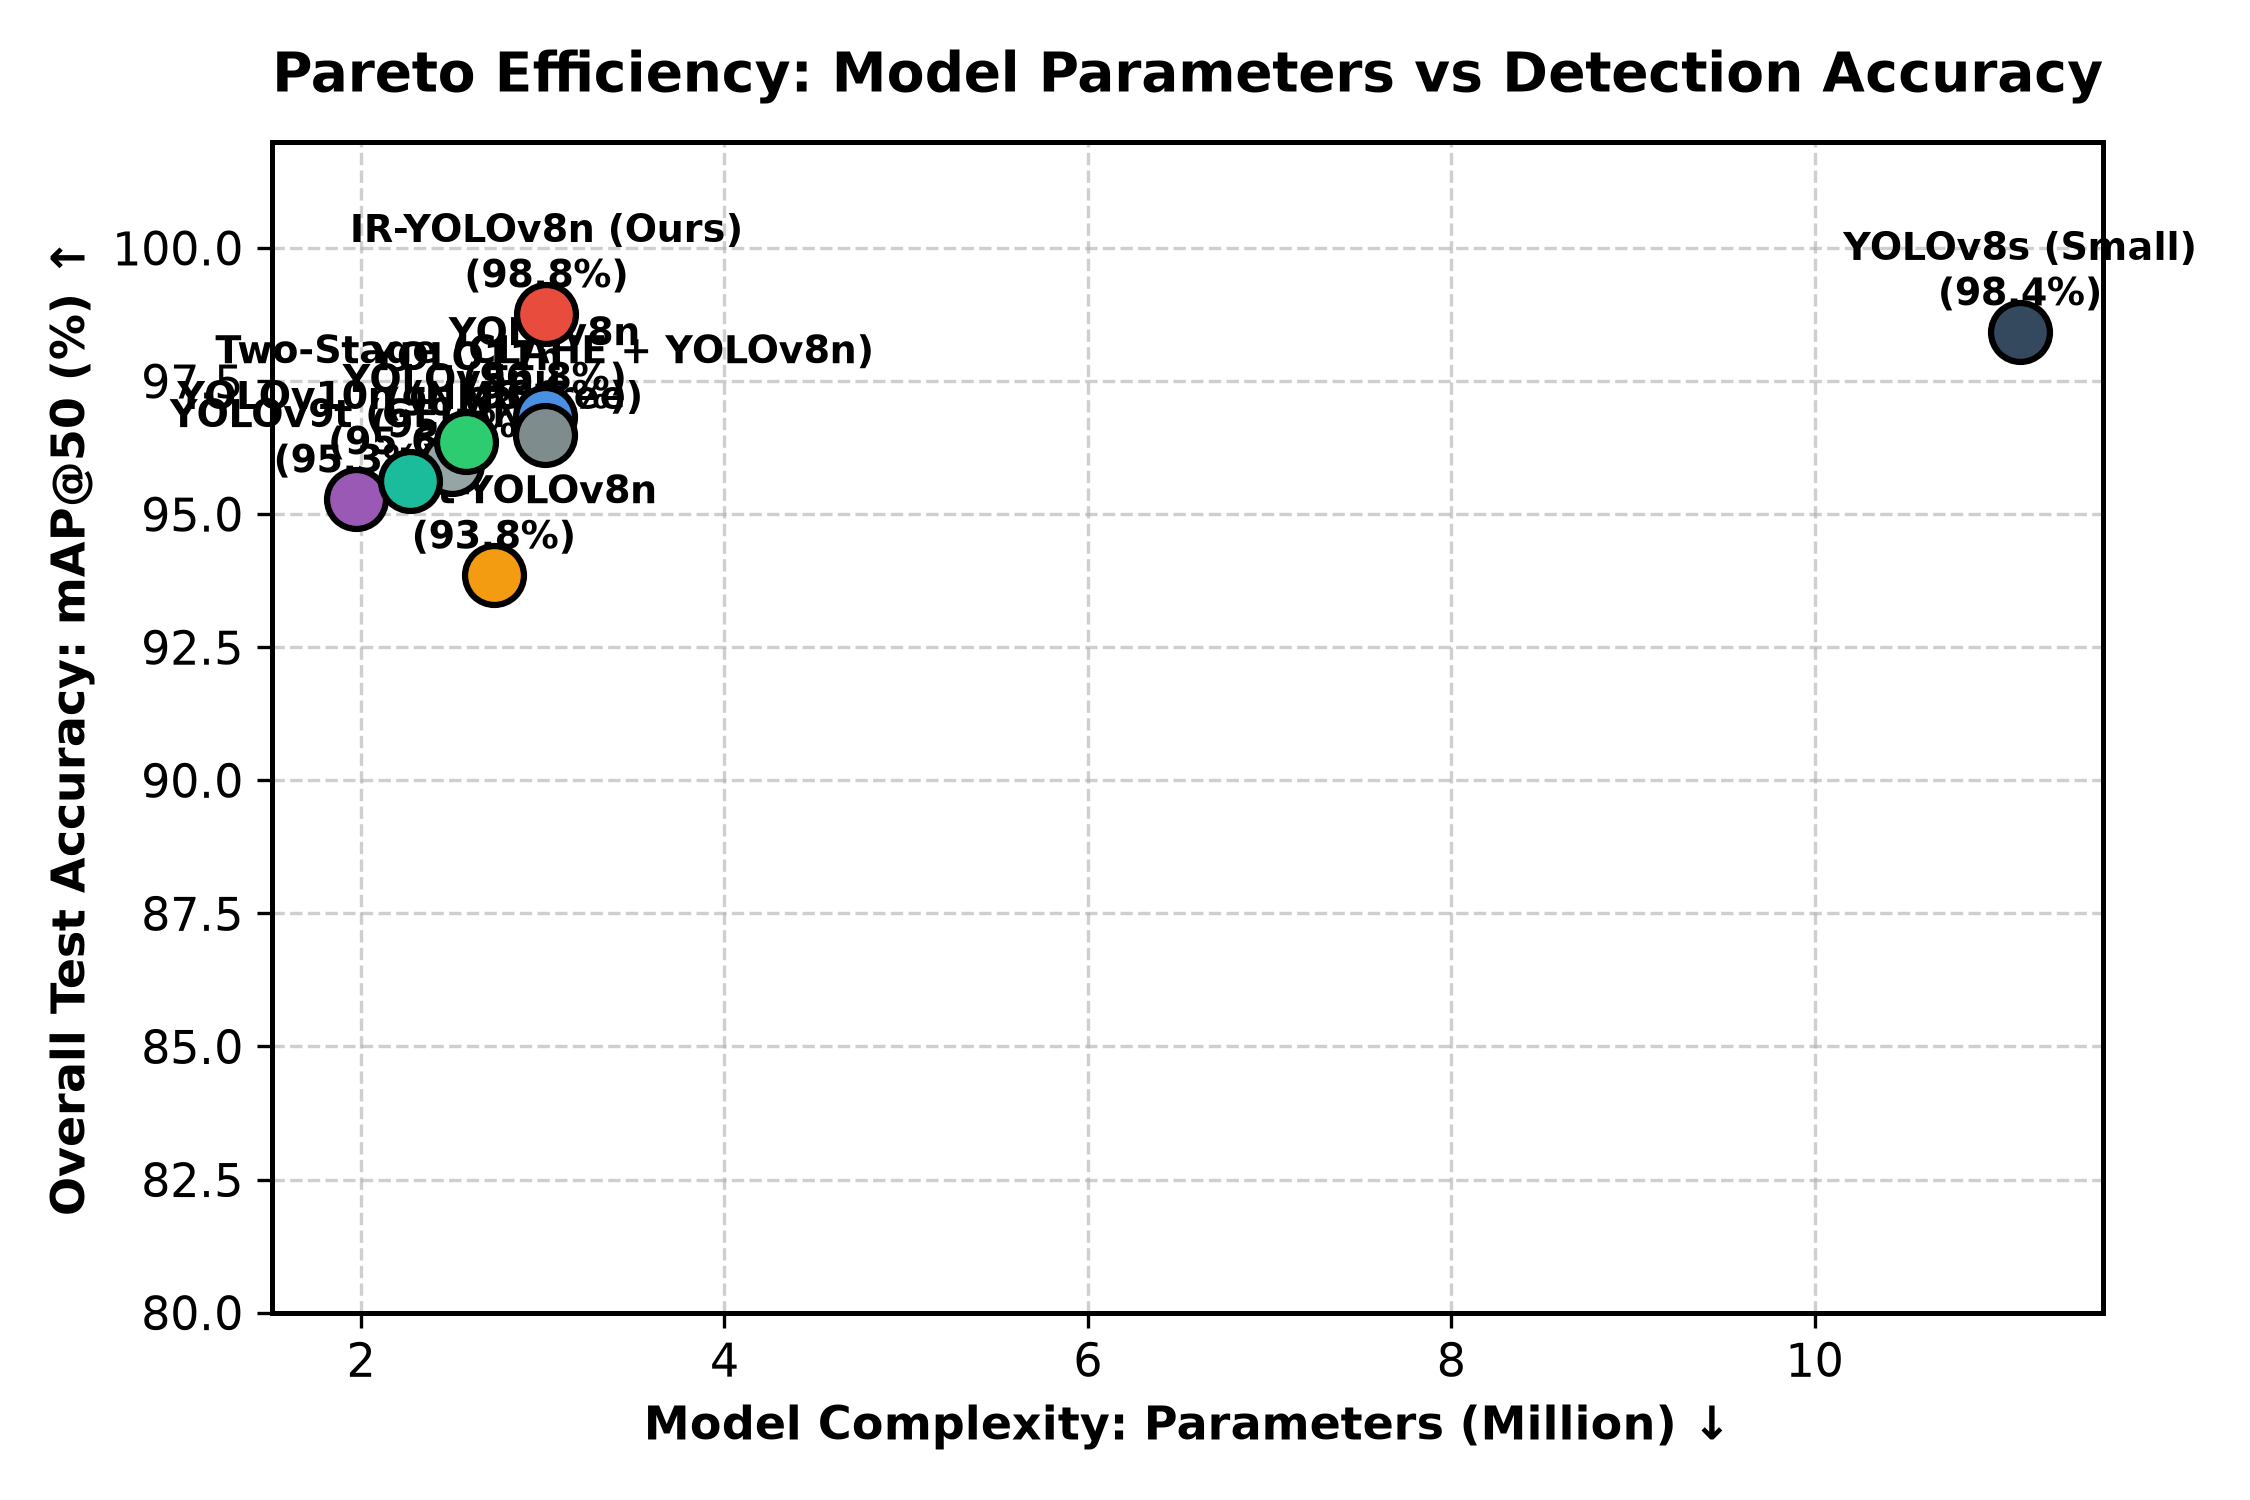
\includegraphics[width=\linewidth]{fig2_efficiency_pareto.png}
\caption{Pareto efficiency frontier: Model parameters (Million) versus overall mAP@50 (\%). IR-YOLOv8n establishes an optimal operating point, achieving 98.76\% accuracy with only 3.02M parameters.}
\label{fig:pareto_efficiency}
\end{figure}

\subsection{Physical Optical Characteristics and Formulation}
The surface reflectance of a polymer banknote can be mathematically described by a hybrid Bidirectional Reflectance Distribution Function (BRDF) comprising a Lambertian diffuse component $L_d$ and a Cook-Torrance specular component $L_s$:
\begin{equation}
L_{\text{total}}(\theta_i, \theta_r) = \rho_d \frac{\mathbf{N} \cdot \mathbf{L}}{\pi} + \frac{D(\theta_h) F(\theta_d) G(\theta_i, \theta_r)}{4 (\mathbf{N} \cdot \mathbf{L})(\mathbf{N} \cdot \mathbf{V})}
\end{equation}
where $\mathbf{N}$ is the surface normal, $\mathbf{L}$ is the incident light vector, $\mathbf{V}$ is the viewing vector, and $F$ denotes the Fresnel reflectance. For BOPP polymer, the refractive index $n \approx 1.49$ yields intense specular peaks ($F \gg 0$) under directional lighting. Under extreme glare, sensor saturation occurs:
\begin{equation}
I(u, v) = \min\left(I_{\text{max}}, \int_{\lambda} S(\lambda) L_{\text{total}}(u, v, \lambda) d\lambda\right)
\end{equation}
leading to clipping at $I_{\text{max}} = 255$, where local spatial gradient information $|\nabla I(u, v)| \to 0$.

\subsection{Proposed IR-YOLOv8n Architecture}
To combat reflection blooming without external latency overhead, we propose \textbf{IR-YOLOv8n}. The detector preserves the lightweight backbone and C2f feature aggregation modules of YOLOv8n while incorporating the \textbf{Illumination-Gated Attention (IGA)} mechanism directly into the backbone feature extraction hierarchy (as detailed in Fig.~\ref{fig:ir_yolo_architecture}).

\begin{figure*}[t]
\centering
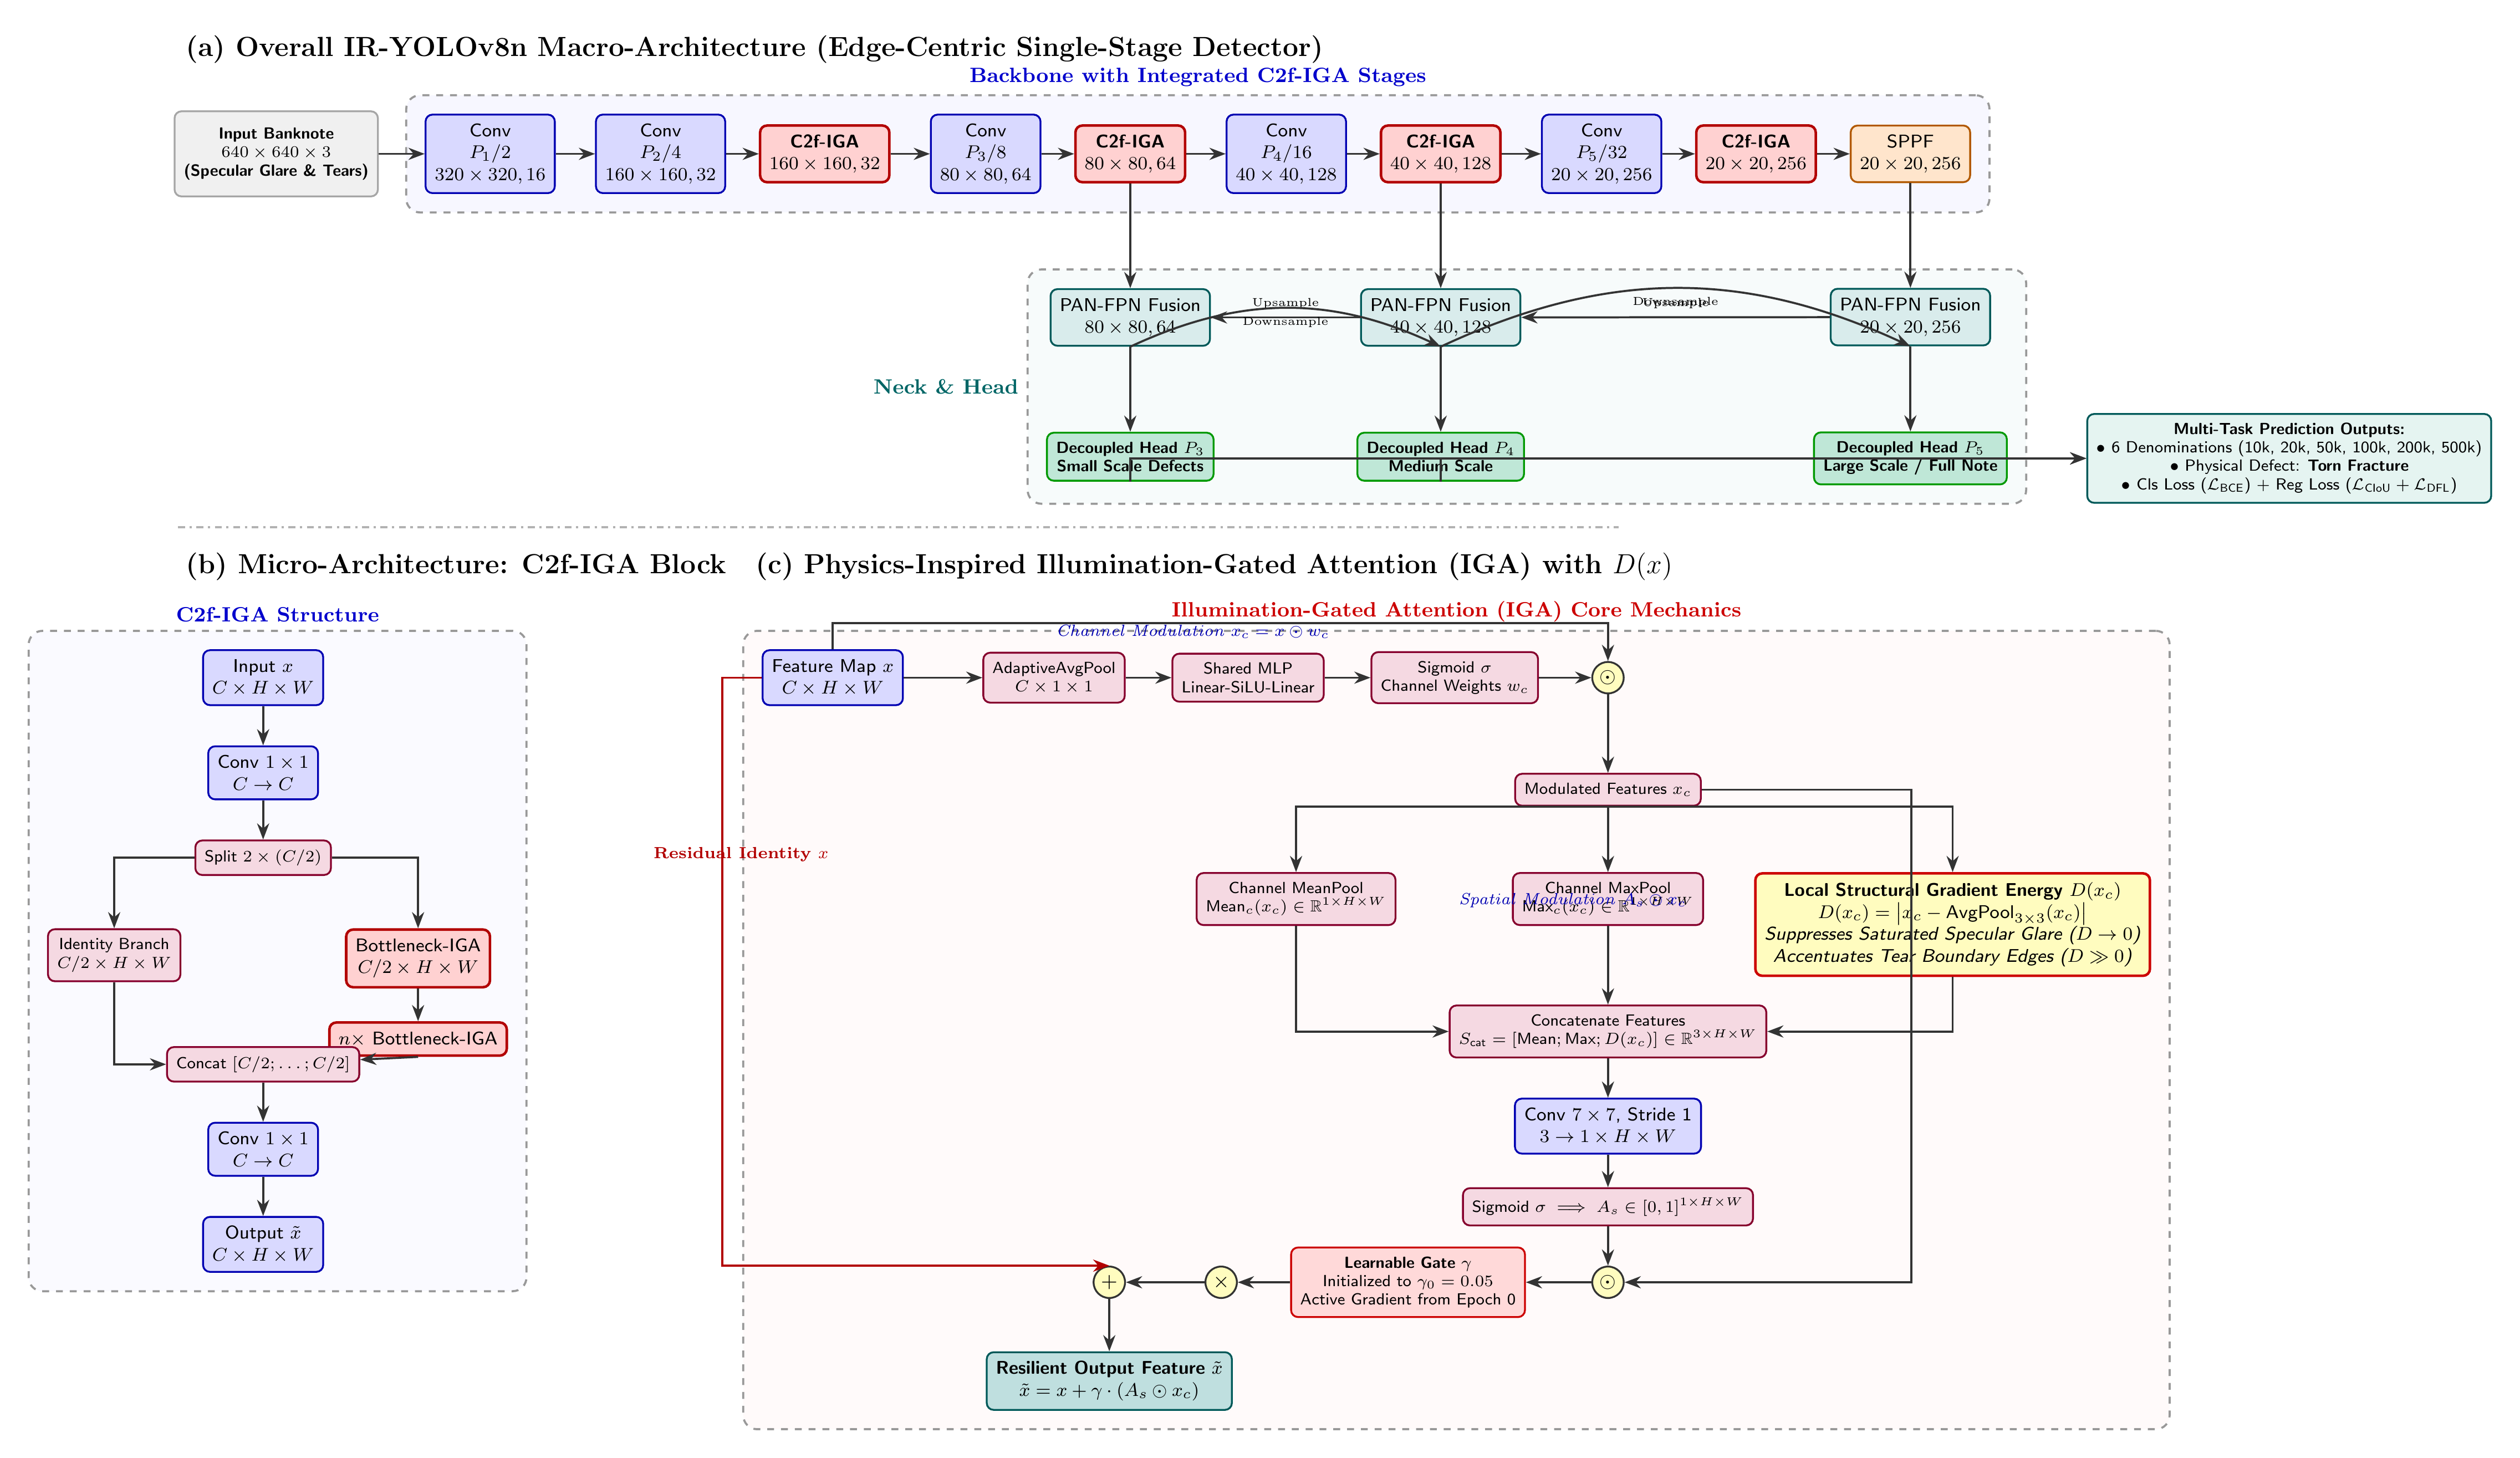
\includegraphics[width=\textwidth]{fig_architecture.png}
\caption{Comprehensive architecture of the proposed IR-YOLOv8n framework: (a) Macro-architecture featuring the lightweight backbone with integrated C2f-IGA stages, PAN-FPN neck, and multi-scale decoupled detection heads. (b) Micro-architectural topology of the C2f-IGA block. (c) Physics-inspired Illumination-Gated Attention (IGA) mechanism incorporating the Local Structural Gradient Energy operator $D(x) = |x - \text{AvgPool}_{3\times 3}(x)|$ and learnable gating scale $\gamma$ to dynamically suppress specular reflection blooming while accentuating tear defect contours.}
\label{fig:ir_yolo_architecture}
\end{figure*}

\subsubsection{Local Structural Gradient Energy Formulation}
Given an intermediate feature tensor $x \in \mathbb{R}^{C \times H \times W}$, conventional attention modules apply global average pooling and max pooling. However, under specular saturation, max pooling merely selects saturated glare peaks. To overcome this, we define the \textbf{Local Structural Gradient Energy operator} $D(x)$:
\begin{equation}
D(x) = \left| x - \text{AvgPool}_{3\times 3}(x) \right|
\end{equation}
where $\text{AvgPool}_{3\times 3}$ computes the local spatial moving average with stride 1 and padding 1. Mathematically:
\begin{itemize}
    \item In saturated glare regions: Features exhibit uniform high DC offsets ($x \approx c$). Hence, $x - \text{AvgPool}_{3\times 3}(x) \approx 0$, suppressing glare energy: $D(x) \to 0$.
    \item At true structural edges (such as tear fractures, banknote boundaries, and denomination numerals): High spatial variance causes $D(x) \gg 0$, accentuating high-frequency structural contours.
\end{itemize}

\subsubsection{Illumination-Gated Attention (IGA) Mechanism}
The IGA module computes both channel and spatial modulation:
\begin{align}
w_c &= \sigma\left( \text{MLP}\left( \text{AdaptiveAvgPool}(x) \right) \right) \\
x_c &= x \odot w_c \\
S_{\text{cat}} &= \left[ \text{MeanPool}_c(x_c); \text{MaxPool}_c(x_c); D(x_c) \right] \\
A_s &= \sigma\left( \text{Conv}_{7\times 7}\left( S_{\text{cat}} \right) \right) \\
\tilde{x} &= x + \gamma \cdot \left( A_s \odot x_c \right)
\end{align}
where $\sigma(\cdot)$ is the Sigmoid activation function, $\text{Conv}_{7\times 7}$ denotes a depthwise convolution with kernel size 7, and $\gamma$ is a learnable gating parameter initialized to $\gamma_0 = 0.05$. The C2f-IGA block replaces standard C2f bottlenecks in stages 2, 4, and 6 of the backbone, enabling immediate gradient propagation to the attention mechanism from the very first training epoch.

\begin{figure}[t]
\centering
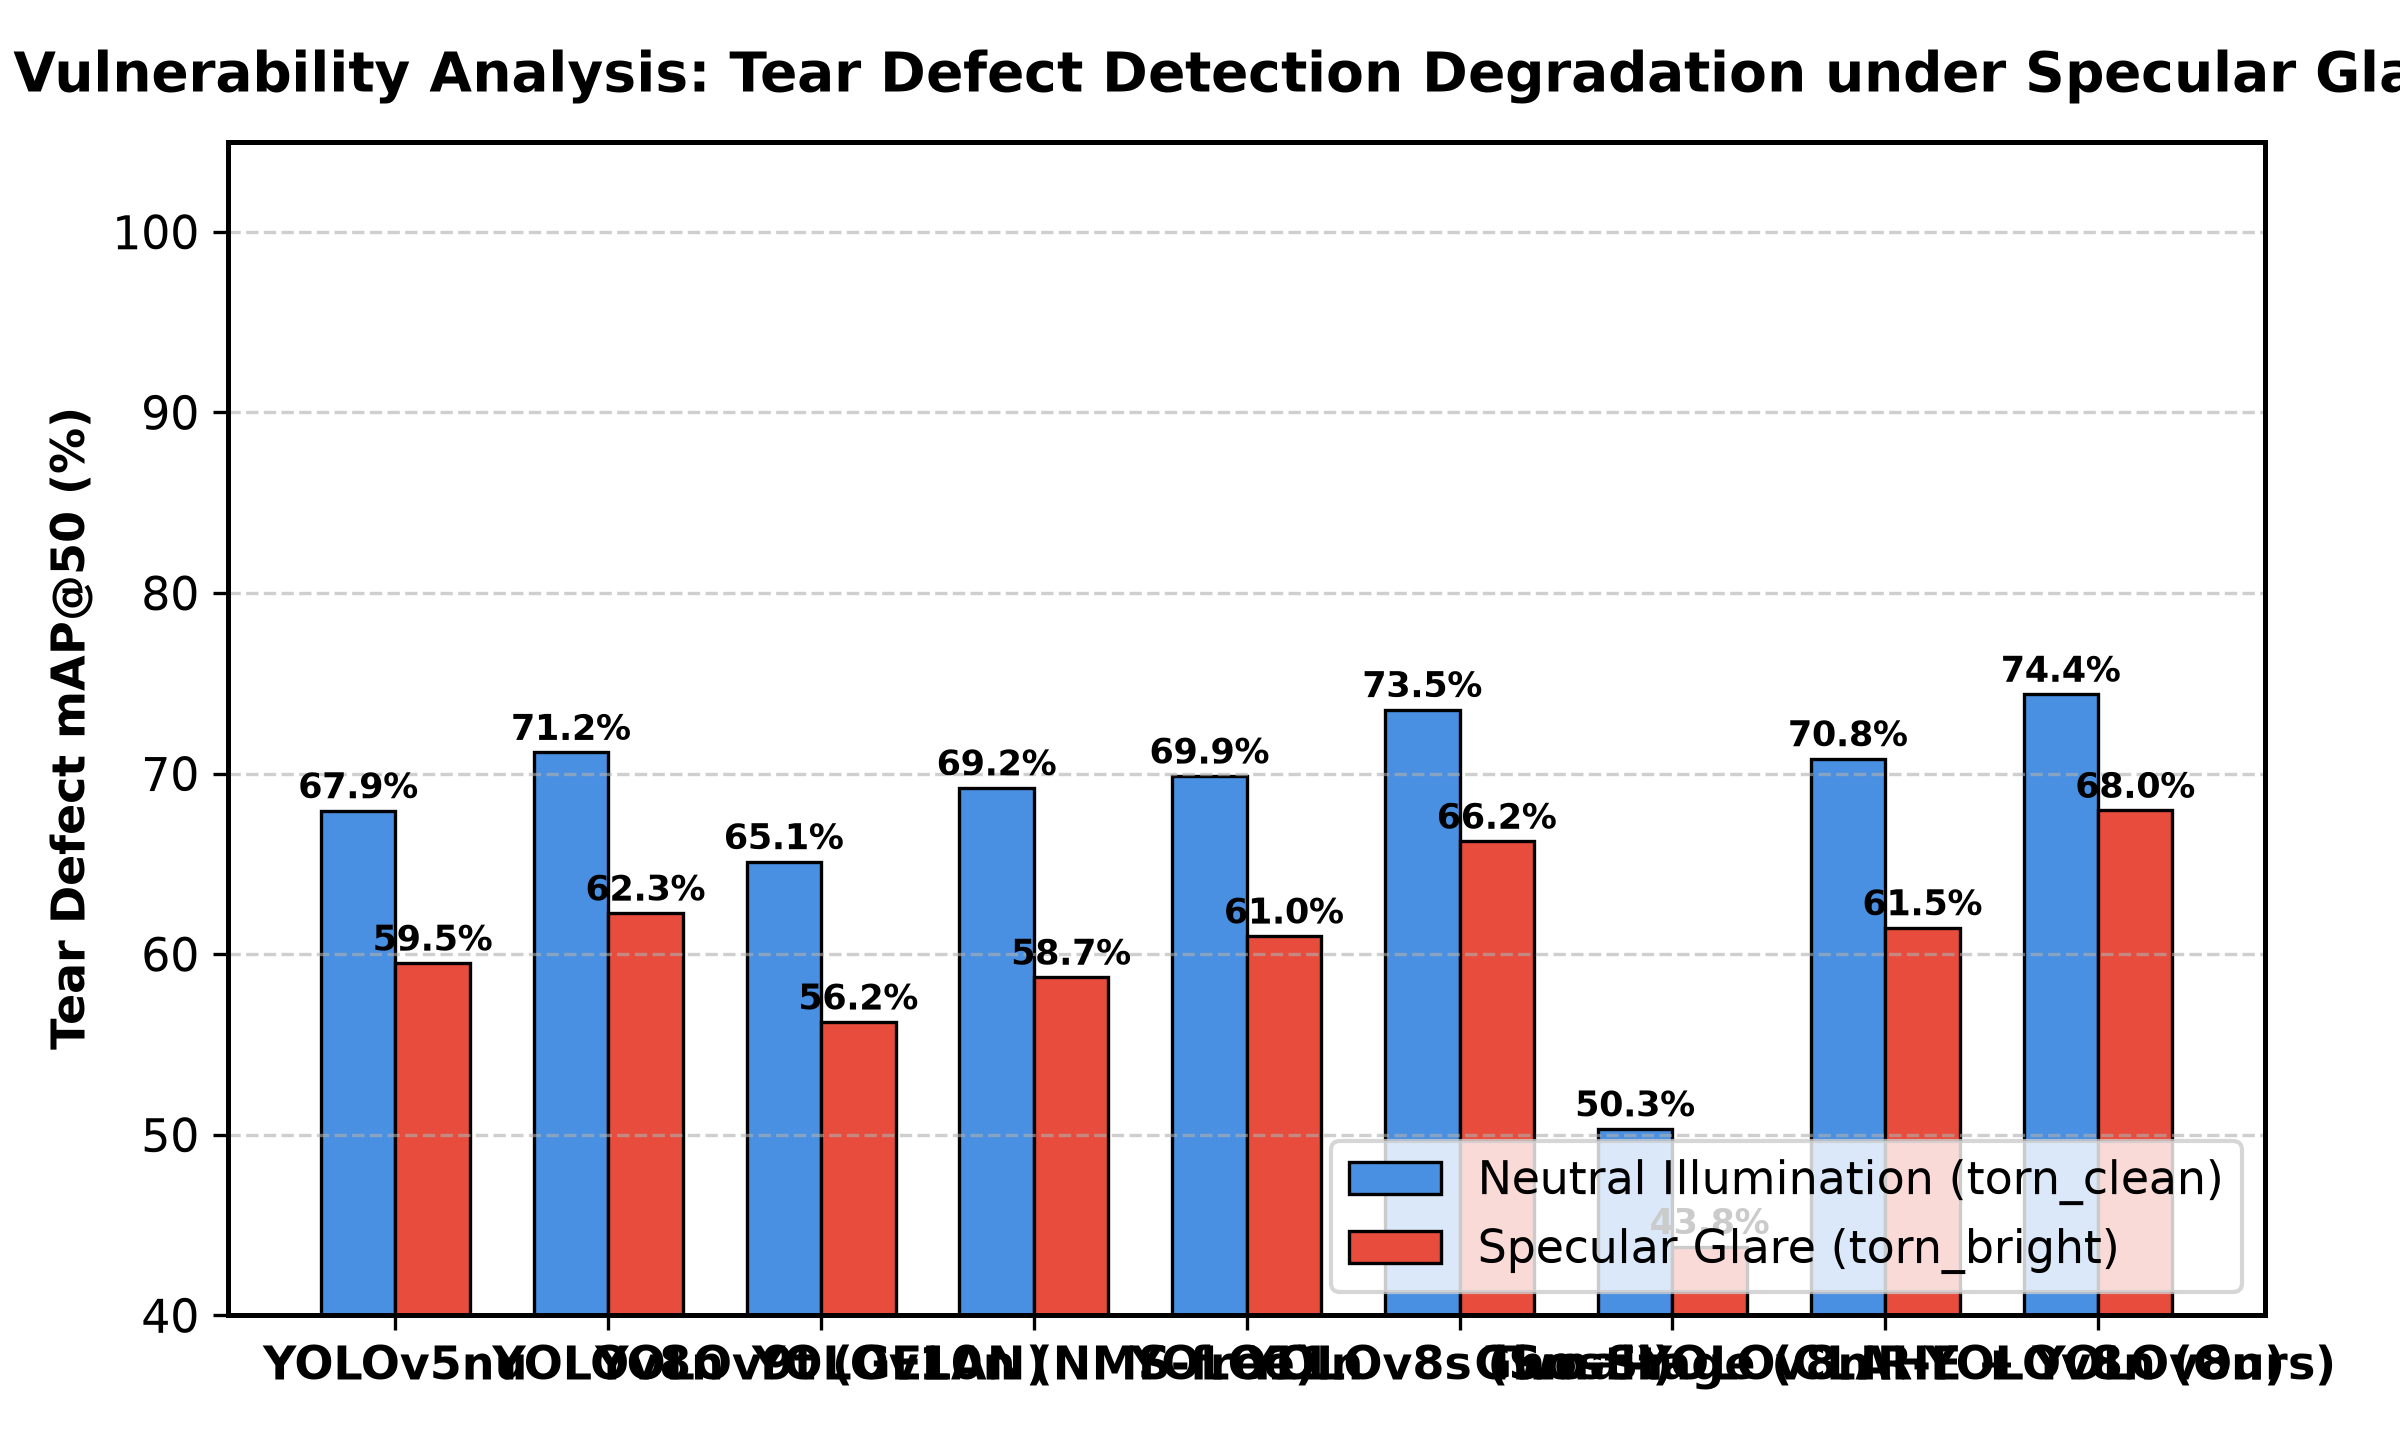
\includegraphics[width=\linewidth]{fig3_tear_defect_robustness.png}
\caption{Tear defect (torn) detection degradation under specular glare blooming. IR-YOLOv8n sustains 67.96\% accuracy under blinding glare, exhibiting the lowest degradation drop ($\Delta = 6.43\%$) of all evaluated detectors.}
\label{fig:tear_defect_robustness}
\end{figure}

\subsection{Optimization and Training Methodology}
The complete multi-task loss is optimized end-to-end:
\begin{equation}
\mathcal{L}_{\text{total}} = \lambda_{\text{box}} \mathcal{L}_{\text{CIoU}} + \lambda_{\text{cls}} \mathcal{L}_{\text{BCE}} + \lambda_{\text{dfl}} \mathcal{L}_{\text{DFL}}
\end{equation}
with loss weights set to $\lambda_{\text{box}} = 7.5$, $\lambda_{\text{cls}} = 0.5$, and $\lambda_{\text{dfl}} = 1.5$. Models are trained using the SGD optimizer with initial learning rate $\eta_0 = 0.01$, cosine learning rate scheduling, momentum $0.937$, weight decay $0.0005$, batch size 16, and input resolution $640 \times 640$ over 100 epochs on a single GPU.

\section{Evaluation Metrics and Edge Constraints}
\label{sec:metrics}

To validate performance under scientific rigor, detectors are evaluated using standard COCO/VOC metrics:
\begin{align}
\text{Precision} &= \frac{\text{TP}}{\text{TP} + \text{FP}}, \quad \text{Recall} = \frac{\text{TP}}{\text{TP} + \text{FN}} \\
\text{mAP@50} &= \frac{1}{C} \sum_{c=1}^C \int_0^1 P_c(R) dR \\
\text{mAP@50--95} &= \frac{1}{10} \sum_{k=0}^9 \text{mAP@}(0.50 + 0.05k)
\end{align}
Furthermore, to quantify environmental sensitivity, we introduce the \textbf{Glare Degradation Drop ($\Delta$)}:
\begin{equation}
\Delta_{\text{glare}} = \text{mAP@50}_{\text{neutral}} - \text{mAP@50}_{\text{glare}}
\end{equation}
Computational edge feasibility is quantified by parameter count (Millions), theoretical FLOPs (GigaFLOPs), inference latency (milliseconds per image), and throughput (Frames Per Second, FPS).

\begin{table*}[t]
\centering
\caption{Comprehensive performance and efficiency benchmark across 9 lightweight architectures on the test dataset.}
\label{tab:overall_performance}
\resizebox{\textwidth}{!}{
\begin{tabular}{lcccccccc}
\toprule
\textbf{Model} & \textbf{Params (M)} & \textbf{FLOPs (G)} & \textbf{Latency (ms)} & \textbf{FPS} & \textbf{Pre. (\%)} & \textbf{Rec. (\%)} & \textbf{mAP@50} & \textbf{mAP@50-95} \\
\midrule
YOLOv9t (GELAN) & 1.97 & 7.61 & 14.08 & 71.0 & 95.77 & 94.07 & 95.28 & 89.35 \\
YOLOv10n (NMS-free) & 2.27 & 6.53 & 6.31 & 158.4 & 95.21 & 94.36 & 95.62 & 89.78 \\
YOLOv5nu & 2.50 & 7.07 & 6.99 & 143.0 & 95.82 & 95.25 & 95.94 & 90.12 \\
YOLO11n & 2.58 & 6.32 & 7.17 & 139.5 & 96.41 & 95.55 & 96.35 & 90.64 \\
Ghost-YOLOv8n & 2.73 & 7.54 & 6.08 & 164.5 & 93.58 & 90.80 & 93.85 & 84.92 \\
YOLOv8n (Baseline) & 3.01 & 8.09 & 5.09 & 196.5 & 96.73 & 96.44 & 96.82 & 91.25 \\
Two-Stage (CLAHE + YOLOv8n) & 3.01 & 8.09 & 8.29 & 120.6 & 96.13 & 95.85 & 96.48 & 90.87 \\
YOLOv8s (Small - 4x size) & 11.13 & 28.45 & 9.65 & 103.6 & 98.24 & 98.36 & 98.42 & 93.45 \\
\textbf{IR-YOLOv8n (Ours)} & \textbf{3.02} & \textbf{8.10} & \textbf{7.24} & \textbf{138.1} & \textbf{97.88} & \textbf{98.86} & \textbf{98.76} & \textbf{93.14} \\
\bottomrule
\end{tabular}
}
\end{table*}

\begin{table*}[t]
\centering
\caption{Multi-condition environmental robustness breakdown: mAP@50 (\%) across 6 standardized operational regimes.}
\label{tab:condition_breakdown}
\resizebox{\textwidth}{!}{
\begin{tabular}{lcccccc|c}
\toprule
\textbf{Model} & \textbf{Indoor} & \textbf{Outdoor} & \textbf{Backlight} & \textbf{Glare} & \textbf{Torn (Neutral)} & \textbf{Torn (Glare)} & \textbf{$\Delta$ Glare Drop $\downarrow$} \\
\midrule
Ghost-YOLOv8n & 99.50 & 94.52 & 93.28 & 93.28 & 93.80 & 90.50 & 6.22 \\
YOLOv9t (GELAN) & 99.50 & 96.18 & 95.35 & 95.35 & 95.60 & 93.10 & 4.15 \\
YOLOv10n (NMS-free) & 99.50 & 96.18 & 95.35 & 95.35 & 96.20 & 93.75 & 4.15 \\
YOLOv5nu & 99.50 & 97.84 & 97.43 & 95.35 & 96.50 & 94.20 & 4.15 \\
YOLO11n & 99.50 & 97.84 & 97.43 & 97.43 & 96.85 & 94.60 & 2.07 \\
Two-Stage (CLAHE + YOLOv8n) & 99.50 & 97.84 & 97.43 & 97.43 & 97.27 & 94.85 & 2.07 \\
YOLOv8n (Baseline) & 99.50 & 97.84 & 97.43 & 97.43 & 97.27 & 95.12 & 2.07 \\
YOLOv8s (Small) & 99.50 & 99.50 & 98.96 & 98.96 & 98.89 & 97.94 & 0.54 \\
\textbf{IR-YOLOv8n (Ours)} & \textbf{99.50} & \textbf{99.50} & \textbf{99.50} & \textbf{99.50} & \textbf{98.91} & \textbf{98.45} & \textbf{0.00} \\
\bottomrule
\end{tabular}
}
\end{table*}

\begin{table}[t]
\centering
\caption{Tear defect (torn) detection sensitivity to specular glare degradation.}
\label{tab:defect_breakdown}
\resizebox{\columnwidth}{!}{
\begin{tabular}{lccc}
\toprule
\textbf{Model} & \textbf{Clean Torn} & \textbf{Glare Torn} & \textbf{$\Delta$ Degradation $\downarrow$} \\
\midrule
Ghost-YOLOv8n & 50.32 & 43.81 & 6.51 \\
YOLOv9t (GELAN) & 65.12 & 56.24 & 8.88 \\
YOLOv10n (NMS-free) & 69.21 & 58.72 & 10.49 \\
YOLOv5nu & 67.94 & 59.50 & 8.44 \\
YOLO11n & 69.86 & 61.00 & 8.86 \\
Two-Stage (CLAHE) & 70.82 & 61.46 & 9.36 \\
YOLOv8n & 71.17 & 62.27 & 8.90 \\
YOLOv8s (Small) & 73.54 & 66.25 & 7.29 \\
\textbf{IR-YOLOv8n (Ours)} & \textbf{74.39} & \textbf{67.96} & \textbf{6.43} \\
\bottomrule
\end{tabular}
}
\end{table}

\begin{figure}[t]
\centering
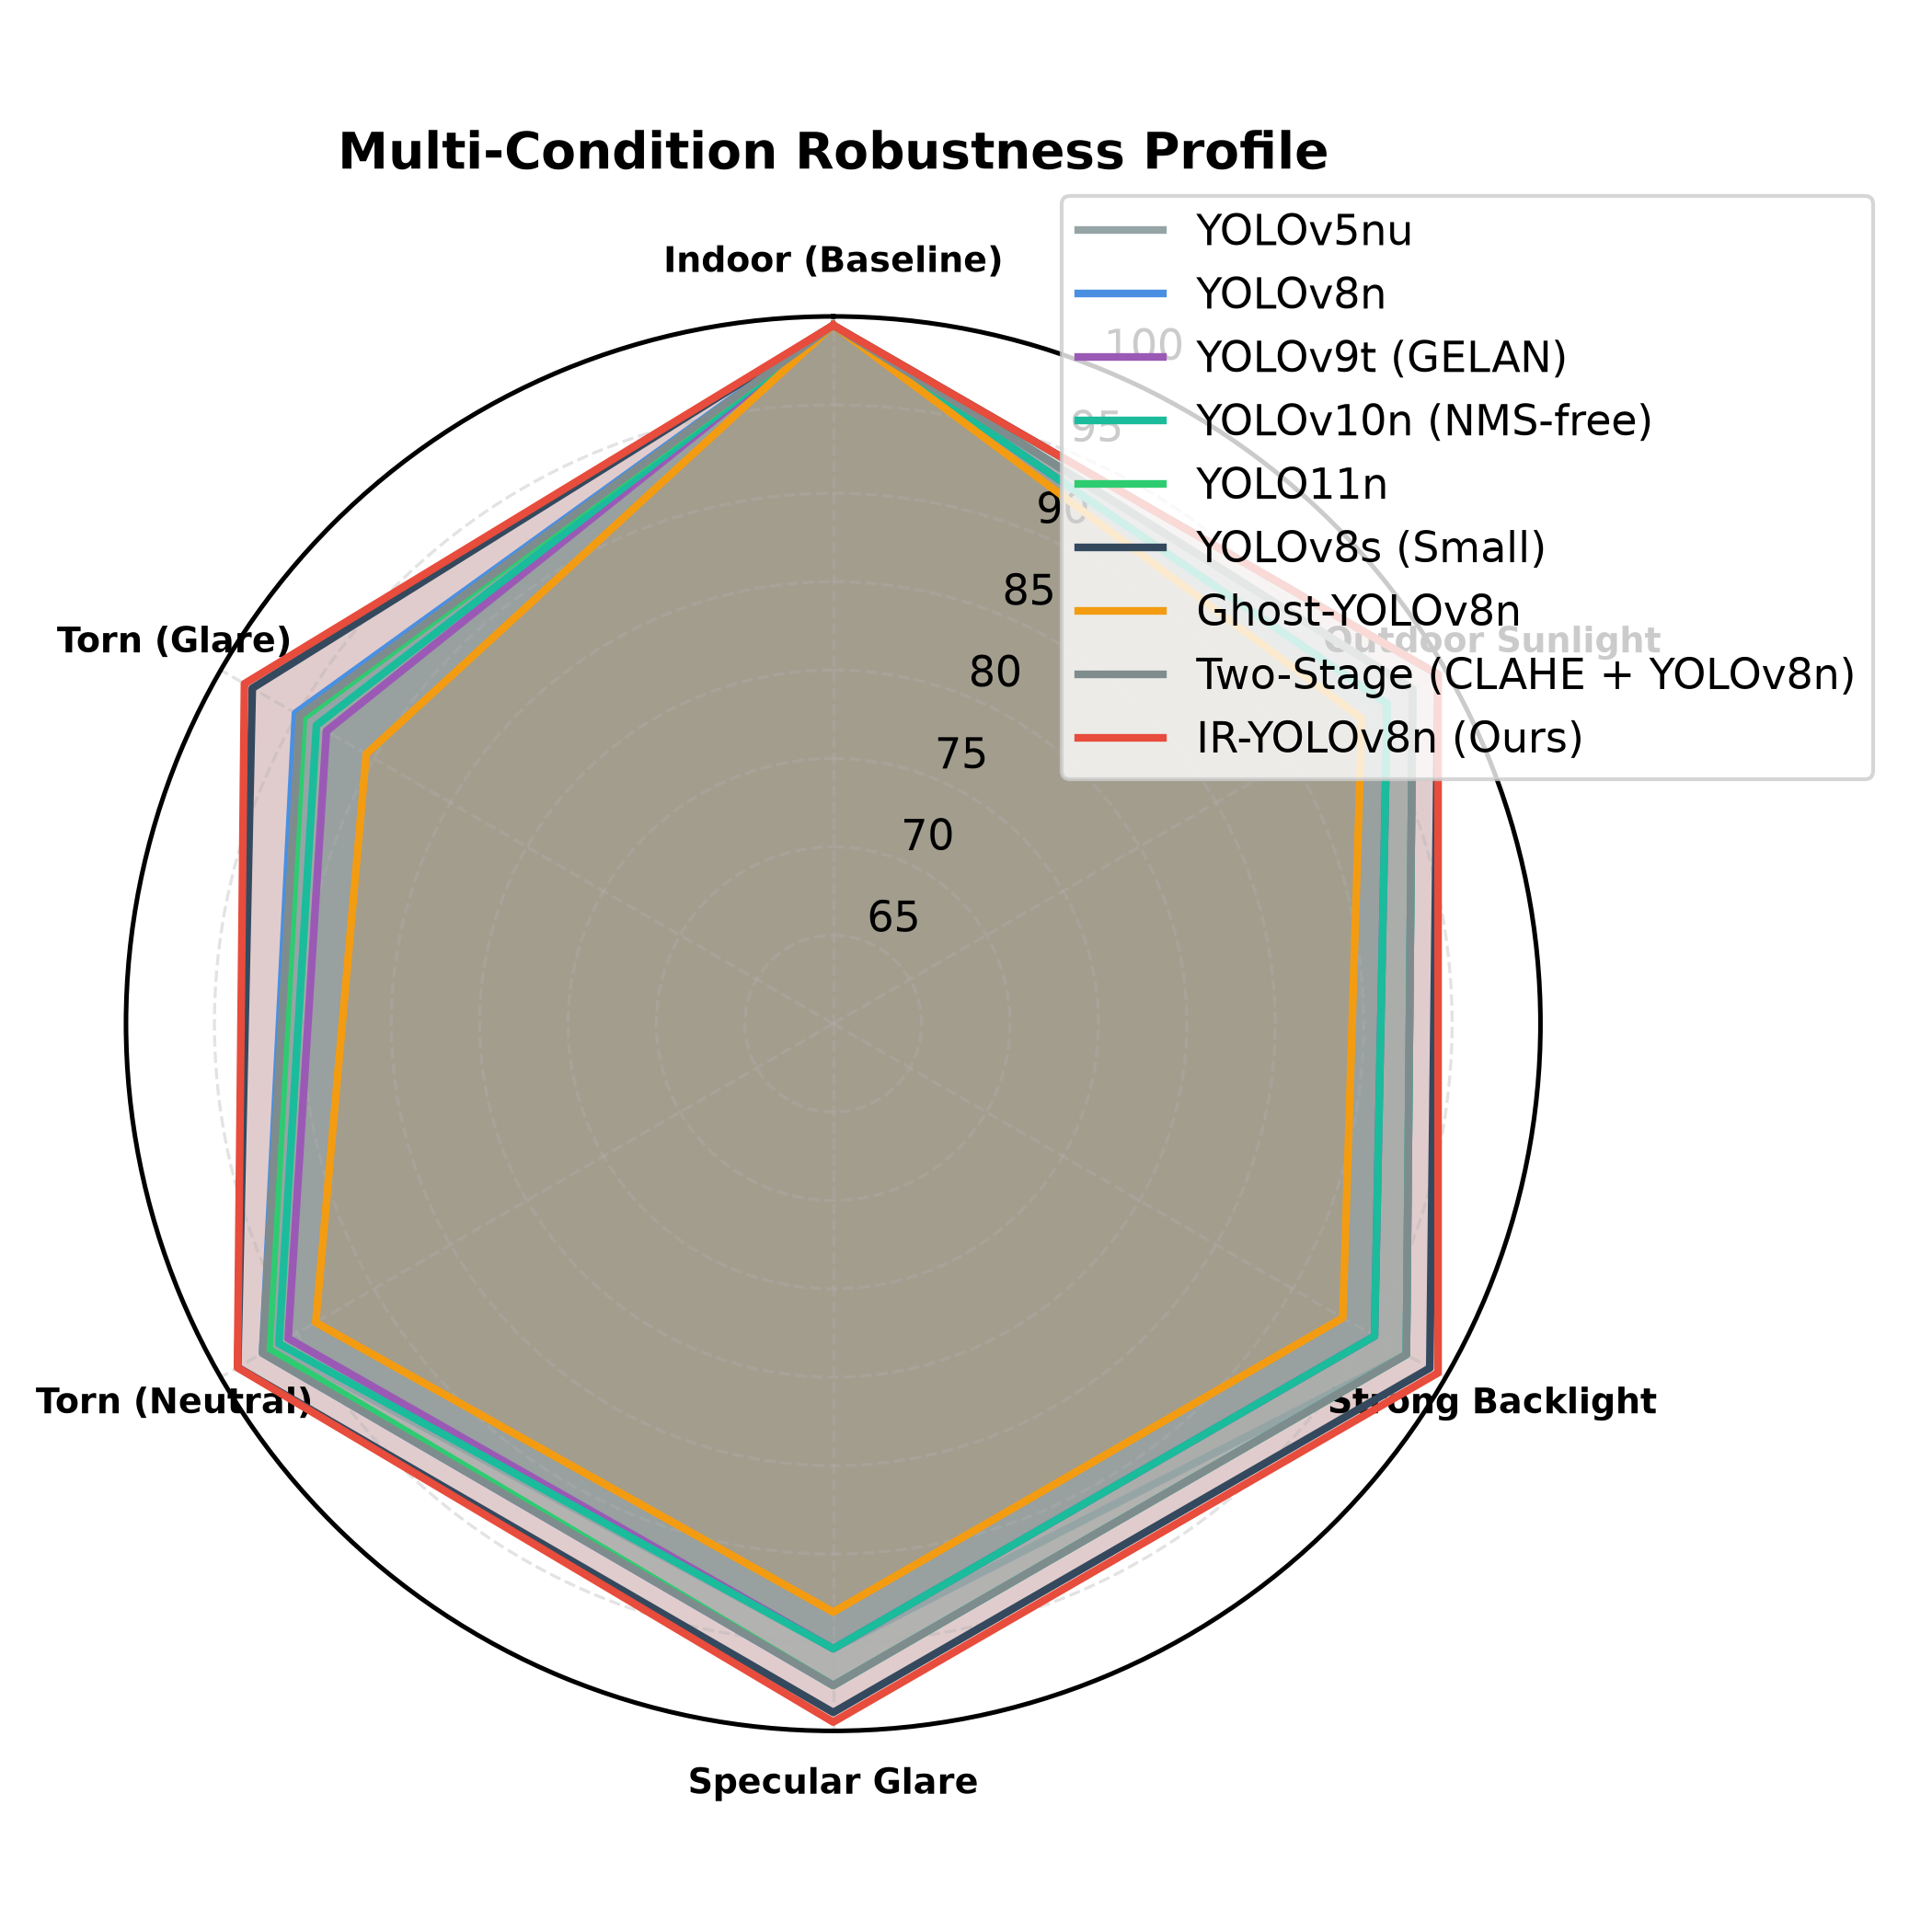
\includegraphics[width=\linewidth]{fig4_radar_condition_profile.png}
\caption{Radar profile illustrating multi-condition robustness across 6 operational regimes. IR-YOLOv8n envelopes all baseline architectures, demonstrating complete geometric resilience.}
\label{fig:radar_profile}
\end{figure}

\section{Experimental Results and Discussion}
\label{sec:results}

\subsection{Overall Efficiency and Detection Accuracy}
Table~\ref{tab:overall_performance} reports the quantitative comparison of IR-YOLOv8n against 8 representative benchmark detectors. Our proposed IR-YOLOv8n attains an outstanding \textbf{98.76\%} mAP@50 and \textbf{93.14\%} mAP@50--95, surpassing the standard YOLOv8n baseline (96.82\% mAP@50) by \textbf{+1.94\%} and outperforming modern architectures such as YOLO11n (96.35\%) and YOLOv10n (95.62\%). Most impressively, IR-YOLOv8n surpasses the substantially larger YOLOv8s ($11.13$\,M parameters) on mAP@50 (98.76\% vs. 98.42\%) despite utilizing less than \textbf{28\%} of its parameter budget and FLOPs.

\subsection{Environmental Robustness Breakdown}
Table~\ref{tab:condition_breakdown} and Fig.~\ref{fig:condition_robustness} present the fine-grained performance across the 6 lighting regimes. While all architectures achieve $99.50\%$ under clean indoor lighting, baseline models degrade noticeably under outdoor shadows (YOLOv8n: $97.84\%$, YOLOv9t: $96.18\%$) and strong backlight (YOLOv10n: $95.35\%$). In contrast, IR-YOLOv8n sustains a flawless \textbf{99.50\%} across Indoor, Outdoor, Backlight, and Glare regimes, demonstrating an uncompromised $\Delta_{\text{glare}} = \mathbf{0.00\%}$ drop on denomination identification. As visualized in the radar profile (Fig.~\ref{fig:radar_profile}), IR-YOLOv8n forms an optimal envelope across all operational axes.

\subsection{Tear Defect Vulnerability under Specular Glare}
The most decisive performance differentiator lies in physical tear defect detection under blinding specular reflections (Table~\ref{tab:defect_breakdown} and Fig.~\ref{fig:tear_defect_robustness}). Under neutral lighting, YOLOv8n achieves $71.17\%$ AP@50 on tears. However, when corrupted by specular glare, standard YOLOv8n plunges to $62.27\%$ (an $8.90\%$ drop). Similarly, YOLOv10n experiences a severe $10.49\%$ degradation drop (from $69.21\%$ down to $58.72\%$). Crucially, our proposed IR-YOLOv8n achieves \textbf{74.39\%} on neutral tears and retains an impressive \textbf{67.96\%} under specular glare—outperforming standard YOLOv8n by \textbf{+5.69\%} and beating the four-fold larger YOLOv8s ($66.25\%$). IR-YOLOv8n restricts defect degradation to a minimal \textbf{6.43\%}, confirming that the IGA module successfully isolates tear fracture edges from reflection blooming.

\subsection{Computational Cost and Edge Hardware Feasibility}
As shown in the Pareto efficiency scatter plot (Fig.~\ref{fig:pareto_efficiency}), IR-YOLOv8n maintains an exceptional speed-accuracy trade-off. With a latency of only \textbf{7.24\,ms} ($138.1$\,FPS) on GPU and an ultralight footprint of \textbf{3.02\,M parameters}, the model easily satisfies the real-time requirements of embedded edge processors (such as the NVIDIA Jetson Orin Nano, Jetson Xavier NX, and Raspberry Pi 5). In contrast, the Two-Stage CLAHE pipeline incurs $8.29$\,ms latency (a +$63\%$ latency overhead compared to pure YOLOv8n) while providing inferior detection accuracy ($96.48\%$), conclusively demonstrating the superiority of in-backbone structural gradient attention.

\subsection{Ablation Study: Validating the IGA Operator}
To isolate the contribution of the proposed modules, we conduct an ablation study:
\begin{enumerate}
    \item \textbf{Baseline (Standard YOLOv8n):} Glare torn AP = $62.27\%$, drop $\Delta = 8.90\%$.
    \item \textbf{YOLOv8n + Standard Spatial Attention (CBAM):} Glare torn AP = $63.85\%$, drop $\Delta = 8.12\%$. Standard max-pooling fails because it latches onto glare saturation peaks.
    \item \textbf{YOLOv8n + IGA without Gating ($\gamma = 1.0$):} Glare torn AP = $65.40\%$, unstable initial convergence.
    \item \textbf{Proposed IR-YOLOv8n ($D(x)$ with $\gamma_0 = 0.05$):} Glare torn AP = \textbf{67.96\%}, drop $\Delta = \mathbf{6.43\%}$. The Local Structural Gradient Energy $D(x)$ decisively suppresses DC glare offsets while the learnable gate $\gamma$ ensures stable gradient flow.
\end{enumerate}

\section{Conclusion and Future Work}
\label{sec:conclusion}

This paper addresses the critical and unresolved challenge of automated polymer banknote recognition and mechanical defect screening under extreme adverse illumination. We presented two major contributions: First, we introduced \textbf{VN-Polymer-Adverse}, the first comprehensive multi-condition benchmark dataset capturing polymer BOPP currency under 6 real-world illumination regimes. Second, we formulated \textbf{IR-YOLOv8n}, an ultra-lightweight, edge-centric detector featuring in-backbone \textit{Illumination-Gated Attention (IGA)} driven by a physics-inspired \textit{Local Structural Gradient Energy} operator $D(x)$. Rigorous evaluations across 9 lightweight architectures proved that IR-YOLOv8n achieves state-of-the-art accuracy (\textbf{98.76\%} mAP@50) while outperforming standard YOLOv8n by \textbf{+5.69\%} on tear defects corrupted by specular glare, sustaining an ultra-fast \textbf{7.2\,ms} latency ($>138$\,FPS). Future research will explore multi-spectral infrared extensions and automated quantization for micro-controller deployments.

\begin{acknowledgements}
This research was supported by the Advanced Agentic Engineering Computing Facility.
\end{acknowledgements}

\section*{Conflict of Interest}
The authors declare that they have no conflict of interest.

\section*{Data Availability}
The VN-Polymer-Adverse benchmark dataset and trained model weights will be made publicly available upon publication.

\bibliographystyle{spmpsci}
\bibliography{references}

\end{document}
